\documentclass[12pt, a4paper, oneside]{book}


%------------------------
% IMPORT PACKAGES
%-----------------------
\usepackage{amsthm}
\usepackage{mathtools}
\usepackage{algpseudocode}
\usepackage[chapter]{algorithm}
\usepackage{amssymb}
\usepackage{graphicx}
\usepackage{caption}
\usepackage{fancyvrb}
\usepackage{array}
\usepackage[acronym,toc,nohypertypes={acronym,notation},nonumberlist,automake]{glossaries}
%\usepackage{hyperref}
\usepackage{epigraph}
\usepackage{url}
\def\UrlBreaks{\do\/\do-}
\usepackage{breakurl}
\usepackage[breaklinks]{hyperref}
\expandafter\def\expandafter\UrlBreaks\expandafter{\UrlBreaks%  save the current one
	\do\a\do\b\do\c\do\d\do\e\do\f\do\g\do\h\do\i\do\j%
	\do\k\do\l\do\m\do\n\do\o\do\p\do\q\do\r\do\s\do\t%
	\do\u\do\v\do\w\do\x\do\y\do\z\do\A\do\B\do\C\do\D%
	\do\E\do\F\do\G\do\H\do\I\do\J\do\K\do\L\do\M\do\N%
	\do\O\do\P\do\Q\do\R\do\S\do\T\do\U\do\V\do\W\do\X%
	\do\Y\do\Z}
\usepackage{listings}
\lstset{
    literate={~} {$\sim$}{1}
}
\usepackage[svgnames, table, dvipsnames]{xcolor}
\usepackage{systeme}
\usepackage{cancel}
\usepackage{color}
\usepackage{tikz}
\usepackage{csquotes}

%% remark theoremstyle
%\newtheoremstyle{break}
%{\topsep}{\topsep}%
%{\itshape}{}%
%{\bfseries}{}%
%{\newline}{}%
%\theoremstyle{break}
%\newtheorem{remark}{Remark}[section]

% problem theoremstyle
%\newtheoremstyle{problemstyle}  % <name>
%{10pt}  % <space acbove>
%{10pt}  % <space below>
%{\normalfont} % <body font>
%{}  % <indent amount}
%{\bfseries\itshape} % <theorem head font>
%{\normalfont\bfseries:} % <punctuation after theorem head>
%{.5em} % <space after theorem head>
%{} % <theorem head spec (can be left empty, meaning `normal')>
%\theoremstyle{problemstyle}
%\newtheorem{problem}{Problem}[section] % Comment out [section] toremove section number dependence
%\newtheorem{definition}{Definition}[section]
%\newtheorem{theorem}{Theorem}[section]
%\newtheorem{proposition}{Proposition}[section]
%\newtheorem{remark}{Remark}[section]
%\newtheorem{lemma}{Lemma}[section]
% create command for variance in math mode
%\newcommand{\Var}[1]{\operatorname{Var}\left[#1\right]}
\newtheorem{thm}{Theorem}[section]
\newtheorem{mydef}{Definition}[section]
\newtheorem{myexample}{Example}[section]
\newtheorem{myprop}{Proposition}[section]
\newtheorem{mylemma}{Lemma}[section]

\newcommand{\source}[1]{\caption*{Source: {#1}} }

\renewcommand\textflush{flushright}
\setlength\epigraphwidth{.6\textwidth}

\makeglossaries
\include{Glossary/glossary}

\definecolor{dkgreen}{rgb}{0,0.6,0}
\definecolor{gray}{rgb}{0.5,0.5,0.5}
\definecolor{mauve}{rgb}{0.58,0,0.82}
\definecolor{light-gray}{gray}{0.95}

\lstdefinestyle{mystyle}{
    backgroundcolor=\color{light-gray},
	basicstyle={\small\ttfamily},
	breaklines=true,
	captionpos=b,
	keepspaces=true,            
	numbersep=5pt,             
	showspaces=false,                
	showstringspaces=false,
	showtabs=false,                 
	tabsize=4
}

\lstset{style=mystyle}


\begin{document}

%----------------------------------------------------------------------------------------
% COVER PAGE
%----------------------------------------------------------------------------------------
\pagestyle{empty}
\begin{titlepage}

	\begin{center}
		\normalsize 
			\textsc{Politecnico di Milano}\\
			School of Industrial and Information Engineering\\
			Master of Science in Mathematical Engineering\\

	\end{center}
	\vspace{.6cm}
	
	\begin{figure}[htpb]
		\centering
		
\includegraphics[width=4cm]{Cover/polimi}
	\end{figure}
	\vspace{.6cm}
	
	\begin{center}
		\LARGE
			\textsc{Notarization \\ }
	\end{center}
	\vspace{1.6cm}

	\begin{flushleft}
		\large
		\begin{tabular}{ll}
		Supervisors:    & Prof. Daniele Marazzina      \\
		             		   & Prof. Ferdinando M. Ametrano
		\end{tabular}
		\vspace{1cm}
	\end{flushleft}
	
	\begin{flushright}
		\large
		Master thesis by:\\
		Andrea Brandoli\\
		ID: 842282\\		
	\end{flushright}
	
	\vspace*{\fill}
	\begin{center}
		Academic year 2018-2019
	\end{center}
	
\end{titlepage}


%----------------------------------------------------------------------------------------
% ABSTRACT
%---------------------------------------------------------------------------------------

%% Set page numbers of the introduction to roman  
\frontmatter
\pagestyle{plain}
%\chapter{Abstract}
Notarization of digital documents is traditionally achieved by a trusted certification authority, which represents a single point of failure. Thus, an application built upon a distributed system reaching consensus in a decentralized way, can greatly strengthen such process. In particular the Bitcoin blockchain, as the most reliable among the others, can be used as a notary to prove that a digital document existed prior to a certain time $t$ and in a certain state, a procedure called timestamping. \textit{OpenTimestamps} is an open-source project that aims to be a standard for timestamping. Additionally, it brilliantly solves a scalability issue found in some previous timestamping attempts on blockchain. The aim of this work is to give an explanation of the whole timestamping process, in particular by means of \textit{OpenTimestamps}. Finally, we developed a fully operating timestamping service, extending such protocol to achieve additional features.

%\cleardoublepage
\vspace*{\fill}
\epigraph{\textit{The secret to happiness is freedom \\ and the secret to freedom is courage.}}{Thucydides}
\vspace*{\fill}


%----------------------------------------------------------------------------------------
%	LIST OF CONTENTS/FIGURES/TABLES PAGES
%----------------------------------------------------------------------------------------

\tableofcontents
\listoftables
\addcontentsline{toc}{chapter}{List of Tables}
\listoffigures
\addcontentsline{toc}{chapter}{List of Figures}
\listofalgorithms
\addcontentsline{toc}{chapter}{List of Algorithms}
\printglossaries

\chapter{Abstract}
Notarization of digital documents is traditionally achieved by a trusted certification authority, which represents a single point of failure. Thus, an application built upon a distributed system reaching consensus in a decentralized way, can greatly strengthen such process. In particular the Bitcoin blockchain, as the most reliable among the others, can be used as a notary to prove that a digital document existed prior to a certain time $t$ and in a certain state, a procedure called timestamping. \textit{OpenTimestamps} is an open-source project that aims to be a standard for timestamping. Additionally, it brilliantly solves a scalability issue found in some previous timestamping attempts on blockchain. The aim of this work is to give an explanation of the whole timestamping process, in particular by means of \textit{OpenTimestamps}. Finally, we developed a fully operating timestamping service, extending such protocol to achieve additional features.
\chapter{Acknowledgements}

%----------------------------------------------------------------------------------------
%	THESIS CONTENT - CHAPTERS
%----------------------------------------------------------------------------------------

\mainmatter


\chapter{Introduction}
\label{chpr:intro}

\section{Thesis Structure}
In Chapter \ref{chpr:consensus} we will start presenting the consensus problem in distributed systems: first we will define what a distributed system is and the main reasons in adopting it (Section \ref{sec:distributed-systems}). Then we will get into the consensus problem (Section \ref{sec:consensus-problem}), in particular in the case of an asynchronous network in presence of byzantine (malicious) nodes (Sections \ref{sec:byzantine-generals} and \ref{sec:byzantine-agreement}), also showing a famous impossibility result (Section \ref{sec:impossibility-result}) in that specific case.

\bigskip
\noindent
Chapter \ref{chpr:btc} will delve into the Bitcoin's novel consensus mechanism. We initially think of Bitcoin as an example of eventual consistency, to focus the Nakamoto's clever intuition of relaxing some properties in the definition of consensus to hold only probabilistically (Section \ref{sec:eventual-consistency}). Then we will give an overview of
the main building blocks of the Bitcoin protocol (Section \ref{sec:btc-design}), with a particular interest for the underlying blockchain as a tamper-evident append-only log (Section \ref{sec:transaction-blockchain}). All this effort to completely understand how Nakamoto practically solves the consensus problem in Bitcoin and why this notorious blockchain is immutable.

\bigskip
\noindent
The first two Chapters set the basis for the core of this thesis work, that is one of the few real non-monetary applications of the blockchain technology: notarization of digital documents, presented in Chapter \ref{chpr:notarization}. More specifically we will define what a timestamp is and how the timestamping procedure works (Section \ref{sec:timestamping}). We will also introduce \textit{OpenTimestamps}, an open-source project that aims to be a standard for blockchain timestamping (Section \ref{sec:ots}), providing a step-by-step tutorial of the usage of its main releases (Sections \ref{sec:ots-client} and \ref{sec:ots-web}).

\bigskip
\noindent
Finally, in Chapter \ref{chpr:project}...
\chapter{Distributed Consensus}
\label{chpr:consensus}

\bigskip
\section{Distributed Systems}
With the persistent expansion of technology in the digital age we are going through, distributed systems are becoming more and more widespread.

\bigskip
\noindent
On one side big companies operate on a global scale with thousands of machines deployed all over the world, big data are stored in various data centers and computational power is shared on multi-core processors or computing clusters.

\bigskip
\noindent
On the other side, every day thousands of people withdraw money in a ATM point, a perfect example of distributed system. But simply, just think about a modern smartphone: it can share multiple data on the cloud and contain multiple co-working processing devices.

\bigskip
\noindent
However, there is no a unique formal definition of distributed system. The one that fits better our interest is:
\begin{mydef} {\bf (distributed system)\footnote{\url{https://en.wikipedia.org/wiki/Distributed_computing}}}.
    A distributed system is a system whose components are located on different networked computers, which communicate and coordinate their actions by passing messages to one another. The components interact with one another in order to achieve a common goal. Three significant characteristics of distributed systems are: concurrency of components, lack of a global clock, and independent failure of components.
\end{mydef}

\bigskip
\noindent
Therefore, the main reasons for using distributed systems are:
\begin{itemize}
    \item Scalability: Distributed systems should be scalable with respect to geography, administration or size.
    \item Performance: Compared to other models, distributed models are expected to give a much-wanted boost to performance.
    \item Fault Tolerance: A cluster of multiple machines is inherently more fault-tolerant than a single one.
    \item Reliability: Data is replicated on different machines in order to prevent loss.
    \item Availability: Data is replicated on different machines to minimize latency and grant fast access.
\end{itemize}

\bigskip
\noindent
However, beautiful features like these often have a downside, bringing to light some challenging problems:
\begin{itemize}
    \item Security: Especially when using public networks.
    \item Coordination\footnote{In the fin-tech industry, coordination problems come with various names: consistency, agreement, consensus or Blockchain.}: In public distributed systems coordination problems are prevalent if proper protocols or policies are not in place; agents could be malevolent or malicious.
\end{itemize}
Thus, it can be easily inferred that one of the main challenges of distributed systems is to achieve overall system reliability in the presence of a number of faulty processes. Examples of applications of consensus include whether to commit a transaction to a database, agreeing on the identity of a leader, state machine replication, clock synchronization, PageRank, load balancing and many others. Let us get in a detailed study of what consensus is and how consensus can be achieved in a distributed system.

\bigskip
\section{The Consensus Problem}
Computers that run programs - nodes - are either \textit{honest}, executing programs faithfully, or \textit{byzantine} \cite{Lamport:1982:BGP:357172.357176}, exhibiting arbitrary behavior. We will also use the terms \textit{correct} and \textit{faulty}, but not as alternatives to honest and byzantine. A correct node is an honest node that always eventually makes progress. A faulty node is a Byzantine node or an honest node that has crashed or will eventually crash. Note that honest and Byzantine
are mutually exclusive, as are correct and faulty. However, a node can be both honest and faulty.
\begin{mydef} {\bf (node)}.
    We call a single actor in the system node. In a computer network the computers are the nodes, in the classical client-server model both the server and the client are nodes, and so on.
\end{mydef}
\begin{mydef} {\bf (byzantine node)\footnote{Before the term \textit{byzantine} was coined, the terms Albanian Generals or Chinese Generals were used in order to describe malicious behavior. When the involved researchers met people from these countries they moved, for obvious reasons, to the historic term byzantine.}}.
    A node which can have arbitrary behaviour is called byzantine. This includes \enquote{anything imaginable}, e.g., not sending any massage at all, or sending different and wrong messages to different neighbors, or lying about the input value.
\end{mydef}

\bigskip
\noindent
We assume that each pair of nodes is connected by a link, which is a bi-directional reliable virtual circuit
and therefore messages sent on this link are delivered, eventually, and in the order in which they were sent
(i.e., an honest sender keeps retransmitting a message until it receives an acknowledgment or crashes). A
receiver can tell who sent a message (e.g., using MACs), so a Byzantine node cannot forge a message so it
is indistinguishable from a message sent by an honest node.

\bigskip
\noindent
In the consensus problem nodes run \textit{actors}, that are either \textit{proposers}, each of which proposes a \textit{proposal}, or \textit{deciders}, each of which \textit{decides} one of the proposals. Assuming there exists at least one correct proposer
(i.e., a proposer on a correct node), the goal of a consensus protocol is to ensure each correct decider decides
the same proposal, even in the face of faulty proposers. A node may run both a proposer and a decider, in
practice a proposer often would like to learn the outcome of the agreement.
\begin{mydef} {\bf (consensus)}.\label{def:consensus}
    There are $n$ nodes, of which at most $f$ might crash, i.e., at least $n-f$ nodes are correct. Node $i$ starts with a proposed value $v_{i}$. The nodes must decide for one of those values, satisfying the following properties:
    \begin{itemize}
        \item Agreement: All correct nodes decide for the same proposal.
        \item Termination: All correct nodes terminate in finite time.
        \item Validity: The decision value must be the proposal of some proposer.
    \end{itemize}
\end{mydef}

\bigskip
\noindent
What is really interesting is to learn how to achieve distributed consensus in an asynchronous network in presence of byzantine nodes. Starting with the historical formulation of the problem and a first example of solved consensus in a model that is synchronous, we will finally face a famous impossibility result in the asynchronous case.

\bigskip
\subsection{The Byzantine Generals' Problem}
Distributed computer systems that want to be reliable must handle faulty components that give conflicting information to different parts of the system.

\bigskip
\begin{center}
	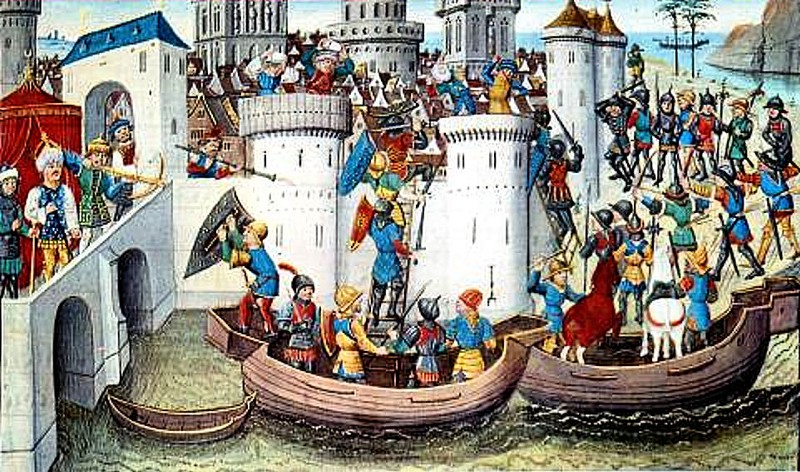
\includegraphics[width=0.9\linewidth]{Images/byzantine.jpeg}
	\captionof{figure}{Conquest of Constantinople}
	\label{fig:figure4}
	\source{\url{https://medium.com/all-things-ledger/the-byzantine-generals-problem-168553f31480}}
\end{center}

\bigskip
\noindent
The \enquote{Byzantine Generals' Problem} is the abstraction of the aforementioned situation.
We imagine that several divisions of the Byzantine army are camped outside an enemy city, each division commanded by its own general. The generals communicate with one another as well as with all lieutenants only by messenger. After observing the enemy, they must decide upon a common plan of action: the exact time to attack all at once or, if faced by fierce resistance, the time to retreat all at once. The army cannot hold on forever, if the attack or retreat is without full strength then brutal defeat is the only possible outcome. However, some of the generals may be traitors, trying to prevent loyal generals from reaching agreement. 

\bigskip
\noindent
For simplicity, we can restrict ourselves to the case of a commanding general sending an order to his lieutenants, obtaining the following problem.
\begin{mydef}{\bf (byzantine generals' problem)}.
\label{def:bgp}
    A commanding general must send an order to his $n-1$ lieutenant generals such that the following conditions\footnote{Conditions \ref{cond:1} and \ref{cond:2} are called the \textit{interactive consistency} conditions} are satisfied:
    \begin{enumerate}
        \item \label{cond:1} All loyal lieutenants obey the same order.
        \item \label{cond:2} If the commanding general is loyal, then every loyal lieutenant obeys the order he sends.
    \end{enumerate}
\end{mydef}

\bigskip
\subsection{Byzantine Agreement}
Achieving consensus (as in Definition \ref{def:consensus}) in a system with byzantine nodes is hard stuff. A careful reader immediately realizes that fulfilling agreement and termination is straight-forward, but what about validity? Reminding that a byzantine node can be malevolent lying about its input value, we must specify different types of validity:
\begin{mydef}{\bf (any-input validity)\footnote{This is the validity definition we implicitly used for consensus, in Definition \ref{def:consensus}}}.
    The decision value must be the proposed value of any node.
\end{mydef}
\noindent
As we can see, this definition does not still make sense in presence of byzantine nodes; we would wish for a differentiation between byzantine and correct inputs.
\begin{mydef}{\bf (correct-input validity)}.
    The decision value must be the proposed value of a correct node.
\end{mydef}
\noindent
Fulfilling this particular validity definition is not so simple, as byzantine nodes following correctly a specified protocol but lying about theirs input values are indistinguishable from correct nodes. An alternative could be:
\begin{mydef}{\bf (all-same validity)}.
    If all correct nodes start with the same proposed value $v$, the decision value must be $v$.
\end{mydef}
\noindent
Here, if the decision values are binary, then correct-input validity is induced by all-same validity. Else, if the input values are not binary, all-same validity is not useful anymore.

\bigskip
\noindent
Now that we have clear in mind what are the ingredients for the consensus recipe, a question bales to us: which are the algorithms that solve byzantine agreement? What type of validity they fulfill? The King algorithm is one of the best examples, but we have to restrict ourselves to the so-called synchronous model.
\begin{mydef}{\bf (synchronous model)}.
    In the synchronous model, nodes operate in synchronous rounds. In each round, each node may send a message to the other nodes, receive the message sent by the other nodes, and do some local computation.
\end{mydef}

\begin{algorithm}
	\caption{King Algorithm (for $f<n/3$)}
	\label{alg:king}
	\begin{algorithmic}[1]
		\State $x =$ my input value
		\For {phase $= 1$ to $f+1$}
		\Statex \ \ \ \ \textit{Round 1}
		\State Broadcast $value(x)$
		\Statex \ \ \ \ \textit{Round 2}
		\If {some $value(y)$ at least $n-f$ times}
		\State Broadcast $propose(y)$
		\EndIf 
		\If {some $propose(z)$ received more than $f$ times}
		\State $x=z$
		\EndIf
		\Statex \ \ \ \ \textit{Round 3}
		\State Let node $v_{i}$ be the predefined king of this phase $i$
		\State The king $v_{i}$ broadcasts its current value $w$
		\If {received strictly less than $n-f$ $propose(x)$}
		\State $x=w$
		\EndIf
		\EndFor
	\end{algorithmic}
\end{algorithm}

\newpage

\bigskip
\noindent
To be rigorous, we must state some useful lemmas in order to prove that Algorithm \ref{alg:king} solves byzantine agreement.
\begin{mylemma}
    \label{lemma:1}
    Algorithm \ref{alg:king} fulfills the all-same validity.
\end{mylemma}
\begin{mylemma}
    \label{lemma:2}
    There is at least one phase with a correct king.
\end{mylemma}
\begin{mylemma}
    \label{lemma:3}
    After a round with a correct king, the correct nodes will not change their values $v$ anymore, if $n > 3f$.
\end{mylemma}

\begin{thm}
    Algorithm \ref{alg:king} solves byzantine agreement.
\end{thm}
\begin{proof}
    The king algorithm reaches agreement as either all correct nodes start with the same value, or they agree on the same value latest after the phase where a correct node was king according to Lemmas \ref{lemma:2} and \ref{lemma:3}. Because of Lemma \ref{lemma:1} we know that they will stick with this value. Termination is guaranteed after $3(f+1)$ rounds, and all-same validity is proved in Lemma \ref{lemma:1}.
\end{proof}

\bigskip
\noindent
However, this is not the end of the story about distributed consensus. In order to dig into the hearth of this work we must introduce consensus results in the asynchronous model.
\begin{mydef}{\bf (asynchronous model)}.
    In the asynchronous model, algorithms are event based (\enquote{upon receiving message ..., do ...}). Nodes do not have access to a synchronized wall-clock. A message sent from one node to another will arrive in a finite but unbounded time.
\end{mydef}
\begin{mydef}{\bf (asynchronous runtime)}.
    For algorithms in the asynchronous model, the runtime is the number of time units from the start of the execution to its completion in the worst case (every legal input, every execution scenario), assuming that each message has a delay of at most one time unit.    
\end{mydef}

\bigskip
\noindent
We will now present a famous algorithm (Algorithm \ref{alg:ben-or}) by Ben-Or \cite{Ben-Or:1983:AFC:800221.806707}, which tries to solve asynchronous byzantine agreement.

\bigskip
\begin{algorithm}
	\caption{Asynchronous Byzantine Agreement (Ben-Or, for $f < n/9$)}
	\label{alg:ben-or}
	\begin{algorithmic}[1]
		\State $x_{i} \in \{0,1\}$ \Comment{input bit}
		\State $r=1$ \Comment{round}
		\State decided = false
		\State Broadcast $propose(x_{i},r)$
		\Repeat
		\State Wait until $n-f$ $propose$ messages of current round $r$ arrived
		\If{at least $n-2f$ $propose$ messages contain the same value $x$}
		\State $x_{i}=x$, decided = true
		\ElsIf{at least $n-4f$ $propose$ messages contain the same value $x$}
		\State $x_{i}=x$
		\Else
		\State choose $x_{i}$ randomly, with $Pr[x_{i}=0] = Pr[x_{i}=1] = 1/2$
		\EndIf
		\State $r=r+1$
		\State Broadcast $propose(x_{i},r)$
		\Until{decided (see Line 8)}
		\State decision = $x_{i}$
	\end{algorithmic}
\end{algorithm}

\bigskip
\noindent
Unfortunately, Algorithm \ref{alg:ben-or} is just a proof of concept that asynchronous byzantine agreement can be achieved, but practically it is unfeasible due to its exponential runtime.

\bigskip
\subsection{Impossibility Result}
A solution to the Byzantine Generals' Problem \ref{def:bgp} may seem a piece of cake. That's not true at all. Its difficulty arises from the fact that if the generals can send only oral messages, then no solution will work unless more than two-thirds of the generals are loyal. An oral message is one whose contents are completely under the control of the sender, so a traitorous sender can transmit any possible message.
Such a message corresponds to the type of message that computers normally send to one another.

\bigskip
\noindent
Let us now show that, if only oral messages are allowed, there is no solution for three generals with a single traitor. For simplicity, the only possible messages that generals can send are \enquote{attack} or \enquote{retreat}. This restriction opens two possible scenarios. In the first scenario, shown in Figure \ref{fig:scenario1}, a loyal commander sends an \enquote{attack} order to his lieutenants, but lieutenant 2 is malevolent and report \enquote{retreat} to lieutenant 1. In this situation, in order to satisfy Condition \ref{cond:2} of problem \ref{def:bgp}, lieutenant 1 must obey the order to attack. In the second scenario, shown in Figure \ref{fig:scenario2}, the commander is a traitor and sends an \enquote{attack} command to lieutenant 1, and a \enquote{retreat} order to lieutenant 2. But, lieutenant 1 does not know who is the traitor and cannot tell the order the commander sent to lieutenant 2. Thus, lieutenant 1 cannot distinguish in which scenario he belongs, so he always obey to the \enquote{attack} order. With a similar argument, if lieutenant 2 receive a \enquote{retreat} order from the commander, he must follow him even if lieutenant 1 reports him to attack. This violates Condition \ref{cond:1} of problem \ref{def:bgp}.

\begin{figure}
\centering
\begin{minipage}{.5\textwidth}
  \centering
  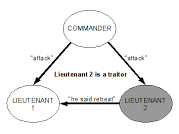
\includegraphics[width=.8\linewidth]{Images/scenario1.png}
  \captionof{figure}{Lieutenant 2 is a traitor}
  \label{fig:scenario1}
\end{minipage}%
\begin{minipage}{.5\textwidth}
  \centering
  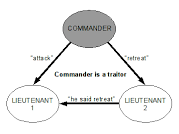
\includegraphics[width=.8\linewidth]{Images/scenario2.png}
  \captionof{figure}{Commander is a traitor}
  \label{fig:scenario2}
\end{minipage}
\source{\url{https://www.researchgate.net/figure/Byzantine-Generals-Problem-Lamport82_fig4_263046309}}
\end{figure}

\bigskip
\noindent
A demanding reader could comply about this nonrigorous result. A famous result\footnote{This result was awarded the 2001 PODC Influential Paper Award (now called Dijkstra Prize).} of Fisher, Lynch and Paterson \cite{Fischer:1985:IDC:3149.214121} formally proves impossibility of distributed consensus with one faulty process.

\bigskip
\noindent
Due to this proven impossibility result, how Satoshi Nakamoto reaches consensus in Bitcoin, a decentralized, distributed, peer-to-peer network? In the next chapter we will delve into this argument.
\chapter{Nakamoto Consensus in Bitcoin}
\label{chpr:btc}
Bitcoin is a distributed, decentralized, peer-to-peer electronic payment system based on cryptographic proof instead of trust, allowing transactions between two counterparts without the need for a trusted third party. However, in late 2008, when the white paper was published by his author Satoshi Nakamoto (metti nota sul nome), it lacked a formalization of the protocol and of the guarantees it claimed to provide.

\bigskip
\noindent
This chapter delves into the core innovation behind Bitcoin, i.e. \textit{Nakamoto consensus}, term that is commonly used to refer to Bitcoin's novel consensus mechanism, which allows mutually distrusting pseudonymous identities to reach eventual agreement.

\bigskip
\section{Bitcoin \& Eventual Consistency}
By its very nature, the Bitcoin network is subject to a type of failure called \textit{network partition}, where a network splits into at least two parts that cannot communicate with each other, often due to software bugs, incompatible protocol versions, or simply network disconnections.
Thus, Bitcoin is inherently characterized by a trade-off between \textit{consistency}, \textit{availability} and \textit{partition tolerance}. Let us be more precise.
\begin{mydef} {\bf (consistency)}.
    All nodes in the system agree on the current state of the system.
\end{mydef}
\begin{mydef} {\bf (availability)}.
    The system is operational and instantly processing incoming requests.
\end{mydef}
\begin{mydef} {\bf (partition tolerance)}.
    Partition tolerance is the ability of a distributed system to continue operating correctly even in the presence of a network partition.
\end{mydef}

\bigskip
\noindent
In practice, only two of these properties can be reached simultaneously; a theorem by Brewer proves this result.
\begin{thm} {\bf (CAP theorem)}.
    It is impossible for a distributed system to simultaneously provide consistency, availability and partition tolerance. A distributed system can satisfy any two of these but not all three.
\end{thm}
\begin{proof}
    Let us assume two nodes that share some state. The nodes belongs to different partitions, so they cannot communicate each other. Assume a request wants to update the state and contacts one of the two nodes. The node may either: 1) update its local state, resulting in a situation of inconsistent states, or 2) not update, resulting in a system no longer available for updates.
\end{proof}

\bigskip
\noindent
Recalling the Definition \ref{def:consensus} of consensus and the properties it must satisfy, a clever intuition of Nakamoto is to weaken the agreement property to hold probabilistically and not deterministically, in order to deal with an asynchronous network. In particular the aforementioned trade-off is in advantage of partition tolerance rather than consistency. In fact, state changes of the underlying transaction ledger (i.e. the blockchain), are rendered probabilistic and the decision on a specific value of the state reaches $Pr(1)$ when $\lim_{r \to \infty}$, where $r$ is the number of rounds in the consensus protocol.

\bigskip
\noindent
Therefore, we can look at Bitcoin as an example of \textit{eventual consistency}.
\begin{mydef}{\bf (eventual consistency)}
    If no new updates to the shared state are issued, then eventually the system is in a quiescent state, i.e., no more messages need to be exchanged between nodes, and the shared state is consistent.
\end{mydef}

\bigskip
\noindent
Now that we have clear in mind the consensus problem in a computer science point of view, we must move forward and study how practically Nakamoto consensus works. Starting from a brief introduction of some basic Bitcoin mechanics we will dig into cryptography concepts and one another innovative idea: economic incentives in a consensus protocol.

\bigskip
\section{Bitcoin Mechanics}

\chapter{Blockchain Notarization with OpenTimestamps}
\label{chpr:notarization}

We devoted Chapter \ref{chpr:consensus} and Chapter \ref{chpr:btc} in understanding how Bitcoin achieves distributed consensus, thus convincing ourselves that the relative blockchain is, in geek speak, \textit{immutable}. We made this effort to lay the foundations for one of the most interesting non-monetary application\footnote{Behind the hype for the blockchain in the current years as the definitive solution of all the world's problems, notarization of digital documents stands out as one of the few real applications of this technology.} of the blockchain, that is the \textit{notarization} of digital documents. According to National Notary Association\footnote{More details in the official website: \url{https://www.nationalnotary.org/knowledge-center/about-notaries/what-is-notarization}.}:

\bigskip
\noindent
\enquote{Notarization is the official fraud-deterrent process that assures the parties of a transaction that a document is authentic, and can be trusted. It is a three-part process, performed by a Notary Public, that includes of vetting, certifying and record-keeping.}

\bigskip
\noindent
Traditionally, the notarization process is achieved by certification authorities (CA), like notary public or banks, because of their reliability. It is only thanks to the relationship of trust with social organizations if this task is possible. The majority of notary services are based on ledgers attesting non-repudiable and non-alterable transactions between two counterparts.

\bigskip
\noindent
However, a central authority represents a single point of failure. Who maintains that ledger could act maliciously and easily tamper some data for his own interest. Hence the need to decentralize the source of trust and grant the reliability of that ledger even if the security of the aforementioned central authority breaks from the inside. A careful reader will have already figured out that the blockchain is the technology that perfectly fits our interest, assuring tamper-resistance and non-repudiation of data written in the chain. Among them, permissionless (public) blockchain is more preferred, because a service built on top of a permissioned (private) blockchain represents a single point of failure, as for a central authority. So, it results that the Bitcoin blockchain is the right answer\footnote{Regarding this, Italian law recognizes the validity of blockchain notarization and AGID will have to specify technical detail. \\ More info here: \url{https://www.agendadigitale.eu/documenti/blockchain-nel-ddl-semplificazioni-conseguenze-e-problemi-dellattuale-testo/}}. Unfortunately, at least for now, it cannot replace all the notary services, but it is perfect to give \textit{proof-of-existance} of a document, a procedure usually called \textit{timestamping}.

\bigskip
\section{Blockchain Timestamping}
\label{sec:timestamping}
A timestamp can be seen as a sequence of characters representing the time in which an event occurred. Hence, timestamping is an increasingly valuable complement to digital signing practices, enabling organizations to record when a digital item, such as a message, document, transaction or piece of software, was signed. In addition, the timing of a digital signature is critical in many cases, like lottery ticket issuance and some legal proceedings. Even when time is not intrinsic to the application, timestamping is helpful for record keeping and audit processes, because it proves whether the digital certificate was valid at the time it was used. More precisely:

\begin{mydef}{\bf (timestamp)}.
    A timestamp is a proof that some data d existed prior to a certain time t.
\end{mydef}

\bigskip
\noindent
To create such proof, $d$ has to cause an event that could not have been
generated without the existence of $d$. Such event must be attested to time $t$ and
can be publicly observed. So a proof consists in the data $d$, the set of operations binding $d$ to the time $t$, and the time attestation. However, we have to deal with the fact that digital documents can be easily falsified without leaving any trail of tamper evidence. Hence, a \enquote{good} timestamp proof must become invalid even if a single bit of the input string is modified. Once again cryptography comes in help and the creation procedure of a timestamp proof does not require to publish $d$ on the blockchain, but only a \textit{commitment} to it, that is something caused by the input $d$ or, in other words, something that follow such input in time. Let us be a little bit more precise:
\begin{mydef}{\bf (commitment operation)}.
    A function $C: X \rightarrow Y$ is a commitment operation if given $x_{1} \in X$ it is not feasible to compute $x_{2} \in X$ s.t. $x_{1} \neq x_{2}, C(x_{1}) = C(x_{2})$.
\end{mydef}

\bigskip
\noindent
Recalling Definition \ref{def:hash-prop}, requiring a function to be a \textit{commitment} operation is the same to require that function to fulfill \textit{second-preimage resistance}, a property already seen in Paragraph \ref{sec:hash} for hash functions. We will now provide some simple examples of commitment operations in order to understand better, the \enquote{\textit{append}} and \enquote{\textit{prepend}} operations.
\begin{myexample}{\bf (\enquote{append})}.
    \textquotedblleft hello\textquotedblright $\xrightarrow{\text{append(\textquotedblleft world\textquotedblright)}}$ \textquotedblleft helloworld\textquotedblright.
\end{myexample}
\begin{myexample}{\bf (\enquote{prepend})}.
    \textquotedblleft world\textquotedblright $\xrightarrow{\text{prepend(\textquotedblleft hello\textquotedblright)}}$ \textquotedblleft helloworld\textquotedblright.
\end{myexample}

\bigskip
\noindent
It is clear that these commitment operations bind inputs to outputs, thus making impossible to tamper the inputs without any evidence in the outputs. However, any user of a timestamp service would have its privacy respected, thus not revealing the content of the data $d$, a property that neither \enquote{\textit{append}} nor \enquote{\textit{prepend}} are able to provide. In addition, the outputs of these specific operations are always bigger in size than the inputs, not a good feature if we want to record such commitments in the blockchain, having blocks strict size limits.

\bigskip
\noindent
To address these issues, we need a tailored commitment operation that fits our case, that is the \textit{hash function}. As we already saw in Paragraph \ref{sec:hash}, hash functions achieve specific properties:
\begin{itemize}
    \item The same input data $d$ will always yield the same hash value.
    \item The hash value is always of a fixed length\footnote{Accordingly to the Bitcoin protocol, we will use SHA256, resulting in a 256-bits output length.}, no matter what size of the input data $d$.
    \item Any change in the input data $d$, even a single bit, will have a totally different hash value and therefore can be detected.
    \item It is impossible to recover the original data $d$ from the hash value, so it hides the input.
\end{itemize}

\bigskip
\noindent
Now that we have seen all the properties a good commitment operation must achieve, what is left is to learn how blockchain timestamp effectively works.

\bigskip
\noindent
Hash functions, like SHA256, are implemented as open algorithms, so any client can \enquote{hash} the document he wants to timestamp from any computer and using any programming languages, without the need to trust any third party for this task.

\bigskip
\noindent
Once the hash value is computed, it can be associated to a particular Bitcoin transaction, called \textit{null data transaction}. This specific type of transaction makes use of OP\_RETURN, an opcode script introduced in the Bitcoin Core 0.9.0 release. It allows to add arbitrary data to a provably unspendable pubkey script that full nodes do not have to store in their UTXO dataset. This feature is good at preventing the UTXO dataset to bloat. From Bitcoin Core 0.11.0, \textit{null data transactions} are relayed and mined with up to 80 bytes\footnote{From version 0.9.x to 0.11.x of the Bitcoin Core, the size for pushing arbitrary data in the null data transaction was 40 bytes.} in a single data push with the limitation of one null data output paying exactly 0 satoshis\footnote{Amounts in Bitcoin are expressed in \textit{satoshi}, currently the smallest unit of the bitcoin currency recorded on the blockchain, i.e. $10^{-8}$ bitcoin.}: 
\begin{verbatim}
Pubkey Script: OP_RETURN <0 to 80 bytes of data>
\end{verbatim}
This \textit{null data script} cannot be spent, so there is not an associated \textit{unlocking script}. Then, the aforementioned transaction is broadcast to the network, waiting for a miner to add it in the transaction set of a mined block. We already saw that a block header contains a specific field called \textit{merkleroot} when we talked about mining in Paragraph \ref{sec:mining-pow}, substantially the root of a binary tree that summarize all the transactions in that block or, in other words, a \textit{commitment} to them. We will use this tree structure, called \textit{merkle tree}\textup{\footnote{The name \textit{merkle tree} comes from Ralph Merkle, who patented it in 1979.}}, in the next chapters, thus we will give here a brief explanation:

\begin{mydef}{\bf (merkle tree)}.
    \label{def:merkle}
    In cryptography and computer science, a binary hash tree or merkle tree is a tree in which every leaf node is labelled with the hash of a data block, and every non-leaf node is labelled with the cryptographic hash of the labels of its two child nodes.
\end{mydef}

\bigskip
\noindent
The simple way to fix in mind such a structure is by a figure. Antonopoulos in his book \enquote{Mastering Bitcoin} \cite{Antonopoulos:2017:MBP:3164842} did it for us.

\begin{figure}[ht]
    \centering
	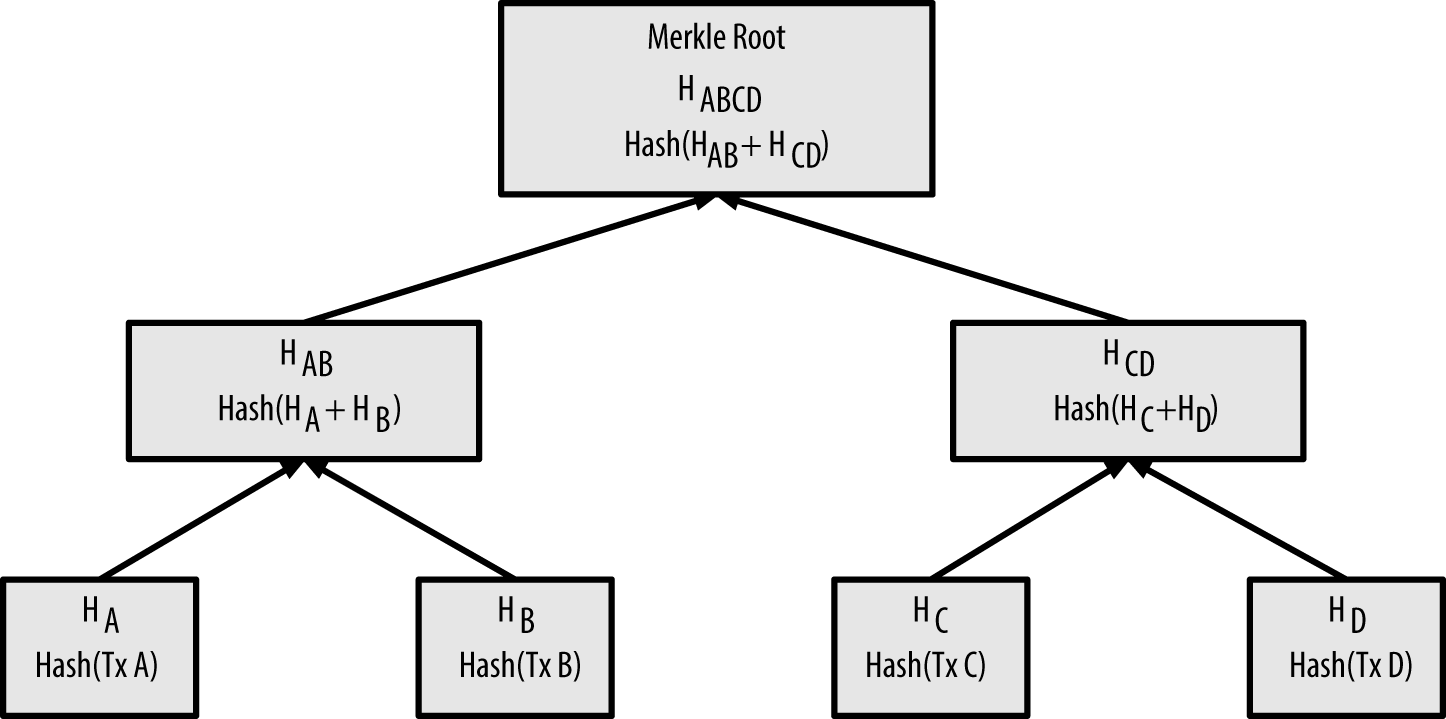
\includegraphics[width=0.9\linewidth]{Images/merkle-tree.png}
	\caption{An example of a merkle tree of transactions}
	\label{fig:merkle}
	\source{\url{https://github.com/bitcoinbook/bitcoinbook/blob/develop/images/mbc2_0902.png}}
\end{figure}

\bigskip
\noindent
A careful reader will already have understood that, in our case, data in Definition \ref{def:merkle} are transactions and the hash function used  is SHA256. Hence, for the properties of hash functions, the \textit{merkleroot}, so the block header commits to all the transactions in a block, also to the specific one that in turn commits to the data to timestamp. 

\bigskip
\noindent
Finally, thanks to what we have learned in the previous chapters, we can think of the Bitcoin network as a decentralized, trustless, permissionless notary. Its attestations are stored in the blockchain, a widely published and immutable timestamps chain\footnote{We recall that a block header also contains a \textit{time} field, a Unix epoch time when the miner started hashing the header (according to the miner). Its value must be strictly greater than the median time of the previous 11 blocks. Full nodes will reject blocks with headers more than two hours in the future according to their clock. This definition is taken from \url{https://bitcoin.org/en/developer-reference\#block-headers}.}. It is this immutability to provide timestamping, proving the data file existence at that moment in time in that specific status.

\bigskip
\noindent
Summing up, blockchain timestamping provides a public proof of existence of a digital document, that cannot be faked or removed and without the need of a central trusted authority. In addition, it can be used along with timestamping prescription. However, this procedure has some downsides, being not efficient (it needs a transaction per timestamp) and lacking a proper standardization. But, in 2012 Peter Todd started working on an open-source project\footnote{The earliest Git commits date back to June 2012, as you can see here: \url{https://github.com/opentimestamps/opentimestamps-server/commit/6e2519d0bb8af2c6ec006e7849d626b20af99a77}.}, called \textit{OpenTimestamps} \cite{OTSWeb}, that aims to provide a standard format for blockchain timestamping, and efficiently resolves these downsides.

\bigskip
\section{OpenTimestamps}
\label{sec:ots}
\textit{OpenTimestamps} defines a set of rules for conveniently creating provable timestamps and later independently verifying them. Currently this protocol fully supports Bitcoin blockchain timestamping, however it is flexible enough to support timestamping on other blockchains like Ethereum and Litecoin. Obviously such a proof is reliable as the chain committing to it, hence without a doubt the Bitcoin one is nowadays the best choice.

\bigskip
\noindent
A timestamp proof made with \textit{OpenTimestamps} consists in a list of commitment operations applied in sequence to the document, ending with one or more time attestations. Such a list of operations is actually a tree of operations, with the document as the root, the commitment operations as the edges and time attestations as the leaves. Anyone can easily verify the proof just replaying the operations and checking that the final result is a message that you already know existed at a certain time. Since commitment operations grant that different inputs will always result in different outputs, we are sure that there is no way to change the original document without invalidating the proof.

\bigskip
\subsection{Solving Scalability Problem}
As we mentioned before, \textit{OpenTimestamps} proposes a solution to the scalability problem, allowing to efficiently aggregate possibly up to an infinite number of documents to timestamp in a single transaction, a feature non supported by most of the existing timestamping services. The trick is to compose those documents in a \textit{merkle tree} and to push its \textit{merkleroot} into a transaction, as the classic blockchain timestamping solutions did for a single hash value. Hence, each per-document proof is just the path up to the first merkle tree composed by documents' hashes, then up to the merkle tree of transactions, reaching the merkleroot in the block header which alone is a commitment to all the documents.

\begin{figure}[ht]
    \centering
	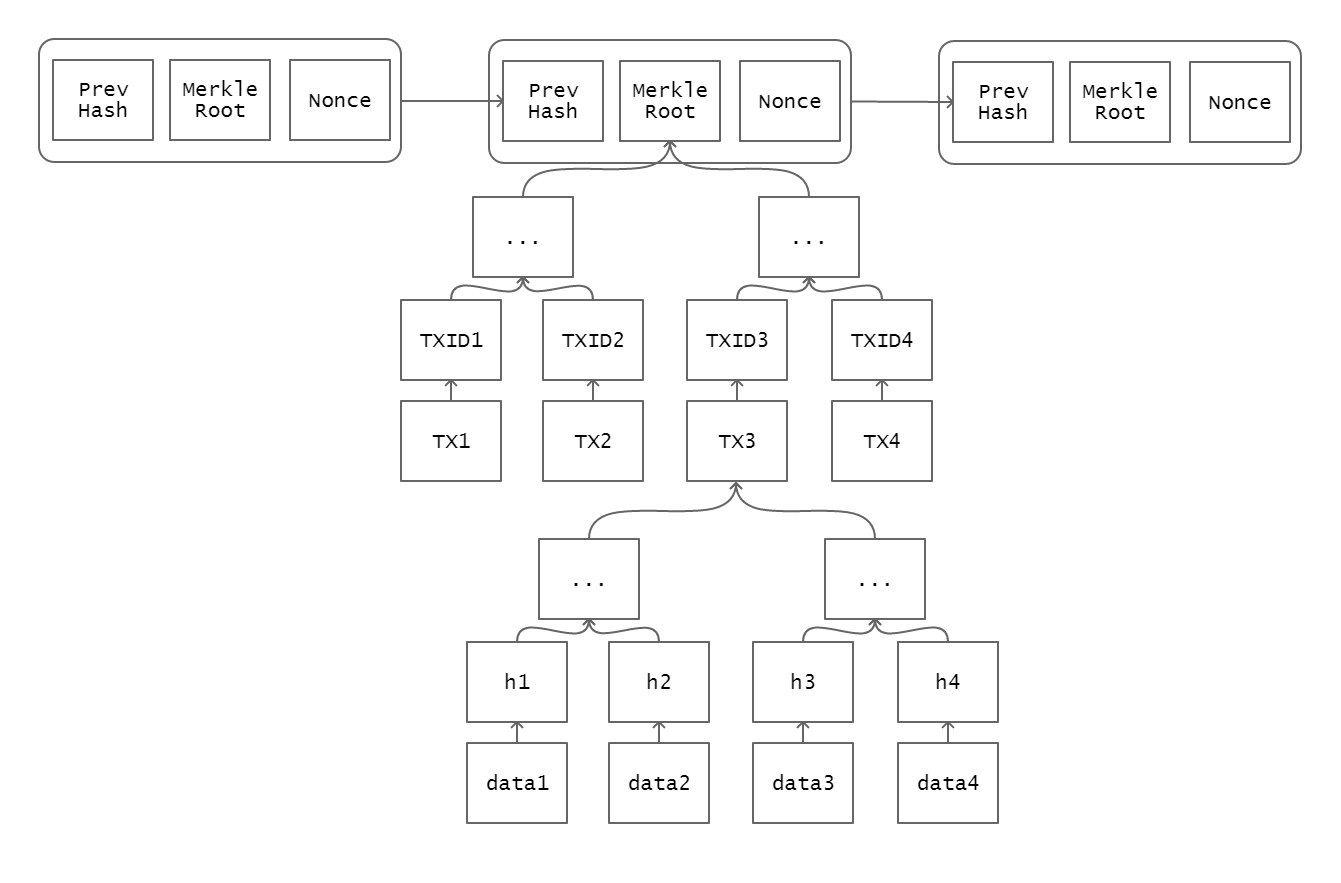
\includegraphics[width=0.9\linewidth]{Images/bitcoin-chain-calendar.png}
	\caption{Scalability solution with \textit{OpenTimestamps}.}
	\label{fig:scalability}
	\source{\cite{Comandini:Thesis:2018}}
\end{figure}

\bigskip
\noindent
In addition to this, \textit{OpenTimestamps} comes with a system of \textit{aggregation servers}\textup{\footnote{Examples of public \textit{aggregation servers} are: \url{a.pool.opentimestamps.org} and \url{b.pool.opentimestamps.org}.}}, publicly available \enquote{meeting points}, where anyone can submit a digest to be timestamped, as Peter Todd said in \cite{OTSannouncment}. As its name suggests, an aggregation server collects documents' hash values in a pending list of digests and periodically \textit{aggregates} these digests into a single merkle tree. Notice that the aggregation server learns nothing about the original documents, it only collects \enquote{meaningless} digests\footnote{In the sense that there is no way to retrieve the original document from its hash value.}. In addition each file is protected by a nonce, thus files are not directly connected in any way. Then, the root of that tree is timestamped with Bitcoin. But there is a little price to pay, aggregation servers are obviously centralized and represent single points of failure because they could go offline, stopping the service. However this represents just a little inconvenience, aggregation servers remain \textit{trustless} in the sense that they cannot tamper a proof, because it is Bitcoin and not theirselves to provide the validity of a timestamp.

\newpage
\noindent
The real downside is that aggregation servers are extremely efficient but not convenient. To obtain a proof, even if for more documents at once, you have to wait for the transaction committing to the document to confirm, that is 10 minutes on average if it is included in the next block. That is too much time in many cases, for example in a timestamped e-mails exchange.

\bigskip
\noindent
But there is a compromise to address this problem which allows any user to receive such proof almost instantly: public \textit{calendar servers}. A \textit{calendar server} grants remote access to a \textit{calendar}, a collection of timestamps. Calendar servers and aggregation servers work in conjunction: rather than timestamping the tip\footnote{We use the word \textit{tip} as a synonym of \textit{root}, hence whenever the word \textit{merkletip} will appear, it indicates the root of that merkle tree.} of the merkle tree of digests directly with Bitcoin, aggregation servers aggregate pending digests in a one second interval into a merkle tree and submit the tip of that tree to a public calendar server. The latter makes the promise that every submitted merkletip will be timestamped by the Bitcoin blockchain in a reasonable amount of time, and keeps indefinitely all completed timestamps, publicly available in every moment. Hence, the proof is generated in about one second. Obviously, the inconvenience here is that public calendar servers are, as aggregation servers before, a central point of failure. In fact, a proof made with the aid of a calendar server is called \textit{incomplete}. However, once the Bitcoin blockchain has definitely completed the timestamp, such incomplete proof can be \textit{upgraded}, adding the path up to the block header merkletip, but we will go into details later in this chapter. Algorithm \ref{alg:calendar-working}, a slight modification of the one proposed by L. Comandini in his master thesis work \cite{Comandini:Thesis:2018}, perfectly describes how calendar and aggregation servers cooperate.

\begin{algorithm}
	\caption{Cooperation between aggregation and calendar servers}
	\label{alg:calendar-working}
	\begin{algorithmic}[1]
		\State clients send data to timestamp to the aggregator\footnotemark \Comment{timestamp requests}
		\State aggregator composes a merkle tree of digests each second\Comment{aggregation}
		\State aggregator sends to calendar the merkletip to timestamp
		\State calendar promise he will timestamp the tip\Comment{pending attestation}
		\State aggregator sends back to clients incomplete proof until the tip
		\State calendar aggregates pending tips in a merkle tree\Comment{aggregation}
		\State calendar sends a transaction including a merkletip\Comment{timestamp}
		\State the transaction gets confirmed \Comment{attestation complete}
		\State clients ask to the calendar to upgrade the timestamp\Comment{upgrade}
		\State calendar sends back clients the complete proofs
		\State clients verify their proofs\Comment{verification}
	\end{algorithmic}	
\end{algorithm}
\footnotetext{The term \textit{aggregator} stands for aggregation server.}

\newpage
\noindent
One last question needs to be answered: who really pays for the transactions in which digests to be timestamped are pushed in? A calendar spends bitcoins from its own wallet, making \textit{replace-by-fee}\textup{\footnote{In Bitcoin, unconfirmed transactions (yet in the mempool) can be modified and re-issued with higher fees for the miners. This leads to a higher probability for that transaction to be mined.}} transactions in order to spend a fixed amount each day. Briefly, the calendar makes a transaction with the lowest possible fees, recursively increasing that amount by a parameter $a$, fixed by who effectively runs the calendar server, until the transaction enters in a block. This result in a fixed amount of $144 \cdot a$ fees spent by the calendar each day, counting a block every 10 minutes on average. It could happen that some timestamps takes too long to be completed, a price that a user willingly pay for a service that allows completely free timestamping.

\bigskip
\noindent
What remains to be done is to learn how to practically timestamp a document with \textit{OpenTimestamps}, which provides users multiple and easy way to create and independently verify timestamps, directly from the official web page \cite{OTSWeb} or with command-line tools. We will now provide a step-by-step guide to use both the web page and the Python version of the client\footnote{\textit{OpenTimestamps} client comes in many programming languages: Python, Java, JavaScript and Rust. Here we present only the Python version because the main reference library of the project is written in Python.}.

\bigskip
\section{OpenTimestamps Python Client}
\label{sec:ots-client}
\textit{OpenTimestamps} client is a command-line\footnote{Here we are supposing a Unix-based operative system.} tool to create and validate timestamp proofs, with the Bitcoin blockchain as a notary. This section is aimed to be a step-by-step tutorial to fully manage the Python release of this client\footnote{The presented guide refers to the Git repository \textit{opentimestamps-client} from the \textit{OpenTimestamps} source code \cite{OpenTimestampsGithub}.}.

\bigskip
\noindent
Before installing the \textit{OpenTimestamps} client, we must specify that while you can \textit{create} timestamps without a local Bitcoin Core node, to \textit{verify} proofs you need one\footnote{For the details about running a Bitcoin node on your local machine, see Appendix \ref{app:A}.} (a pruned node is fine too). Standing the above consideration, the increased difficulty in using a command-line tool rather than a web interface is rewarded by a complete decentralization, you do not have to rely on any third part.

\begin{itemize}
\item Install client (Python3 required):\bigskip
\begin{lstlisting}
 $ pip3 install opentimestamps-client
\end{lstlisting}
\item Install the necessary dependencies:\bigskip
\begin{lstlisting}
 $ sudo apt-get install python3 python3-dev python3-pip python3-setuptools python3-wheel
\end{lstlisting}
\item Pick a file or create a new one to timestamp:\bigskip
\begin{lstlisting}
 $ cat > filename.txt
 bla bla bla ... (write what you want)
 (type CTRL+D to close the file and return to command prompt)
\end{lstlisting}
\item Timestamp your file:\bigskip
\begin{lstlisting}[breakatwhitespace=true]
 $ ots stamp filename.txt 
 Submitting to remote calendar https://a.pool.opentimestamps.org
 Submitting to remote calendar https://b.pool.opentimestamps.org
 Submitting to remote calendar https://a.pool.eternitywall.com
 Submitting to remote calendar  https://ots.btc.catallaxy.com
\end{lstlisting}
Nice! Your timestamp request is submitted to the main public calendar servers.

\bigskip
\noindent
At this time the client must have automatically downloaded in your current directory a file
with a .ots extension, named \colorbox{light-gray}{filename.txt.ots} that is the proof of your timestamp.
\item Verify the proof (local Bitcoin Core node needed):\bigskip
\begin{lstlisting}
 $ ots verify filename.txt.ots 
 Assuming target filename is 'filename.txt'
 Calendar https://bob.btc.calendar.opentimestamps.org: Pending confirmation in Bitcoin blockchain
 Calendar https://alice.btc.calendar.opentimestamps.org: Pending confirmation in Bitcoin blockchain
 Calendar https://btc.calendar.catallaxy.com: Pending confirmation in Bitcoin blockchain
 Calendar https://finney.calendar.eternitywall.com: Pending confirmation in Bitcoin blockchain
\end{lstlisting}
Notice that you can't verify immediately the aforementioned proof. In fact, the lines saying \enquote{pending confirmation} specify that the proof is \textit{incomplete}, so a verifier has to ask the remote calendars for the rest of the proof. It takes a few hours for the timestamp to get confirmed by the Bitcoin blockchain (generally 6 confirmations). You can check for the current status of your proof file with the \colorbox{light-gray}{info} command.
\item Get detailed proof information:\bigskip
\begin{lstlisting}[breakatwhitespace=true]
 $ ots info filename.txt.ots 
 File sha256 hash: 13a1f687ddb7c1a0b12adeb708a2b464c9 cfc24d5c9def4fa775cca81162feed
 Timestamp:
 append 5669aa818cc1c5bf8129d469f884fe79
 sha256
  -> append 0f2a11ae083c66674d9d0d3da049079e
     sha256
     prepend f6836f41e86344eb7e4da03fe57c3e998d13594b2a27b4 ccb86cef8ac19cf69e
     sha256
     prepend 5c502267
     append 2c767f767b02b45c
     verify PendingAttestation ('https://bob.btc.calendar.opentimestamps.org')
  -> append 675406ae56e9e40809ac587ee009067c
     sha256
     append 7690b939b5a663ea311992aadf2f182424cea544bbfb2a 837ae366ba5cc1ecf4
     sha256
     prepend 5c502266
     append 1269e2007cc47092
     verify PendingAttestation ('https://alice.btc.calendar.opentimestamps.org')
  -> append 9b10d7ec7f0af842407d2d7cbebac9ad
     sha256
     prepend 5c502267
     append da1d41ee8803dff5
     verify PendingAttestation ('https://btc.calendar.catallaxy.com')
  -> append f923446e73e3a503121a56006723a6c1
     sha256
     append c35e379ef7097a65fdbfb2a594a93c75
     sha256
     prepend 5c502266
     append c47a3b08bfc2315e
     verify PendingAttestation ('https://finney.calendar.eternitywall.com')
\end{lstlisting}
Incomplete timestamps can be upgraded using the \colorbox{light-gray}{upgrade} command which adds the path to the relative block header merkleroot to the proof. Upgrading a proof isn't always available: there must be at least one completed attestation\footnote{That is, at least one of the four public calendars in question must have received an attestation from the Bitcoin blockchain.}.
\item Upgrade the proof: \bigskip
\begin{lstlisting}[breakatwhitespace=true]
 $ ots upgrade filename.txt.ots 
 Got 1 attestation(s) from https://bob.btc.calendar.opentimestamps.org
 Got 1 attestation(s) from https://alice.btc.calendar.opentimestamps.org
 Got 1 attestation(s) from https://btc.calendar.catallaxy.com
 Got 1 attestation(s) from https://finney.calendar.eternitywall.com
 Success! Timestamp complete
\end{lstlisting}
In this case the timestamp is fully confirmed by the Bitcoin blockchain, so upgrading the proof succeeded.

\bigskip
\noindent
Now that we know for sure that timestamping succeeded, you only left to use the \colorbox{light-gray}{verify} command another time to check which block attested your timestamp (add the flag \colorbox{light-gray}{-v} to be more verbose).\bigskip
\begin{lstlisting}[breakatwhitespace=true]
 $ ots -v verify filename.txt.ots
 Assuming target filename is 'filename.txt'
 Hashing file, algorithm sha256
 Got digest 13a1f687ddb7c1a0b12adeb708a2b464c9cfc24d5c9def 4fa775cca81162feed
 Attestation block hash: 00000000000000000013e603482 1d3d85e8a8ff0217482e4b2ab602ec7ab6ce7
 Success! Bitcoin block 560604 attests existence as of 2019-01-29 CET
\end{lstlisting}
\end{itemize}

\bigskip
\section{OpenTimestamps Web Interface}
\label{sec:ots-web}
Rather than the more complicated client, the easiest way to perform a timestamp with \textit{OpenTimestamps} is using the web interface on the official website \cite{OTSWeb}. It obviously allows the same actions as the client does, just interacting with the \enquote{Stamp \& Verify} box. Simply, drop a file in the box to \textit{stamp} it and the service will automatically download its proof, named as the file is with a \colorbox{light-gray}{.ots} extension. The hash of the document will be calculated inside your browser, thus not requiring the user to distribute his original document to any third party, preserving privacy.

\bigskip
\begin{figure}[htbp]
    \centering
	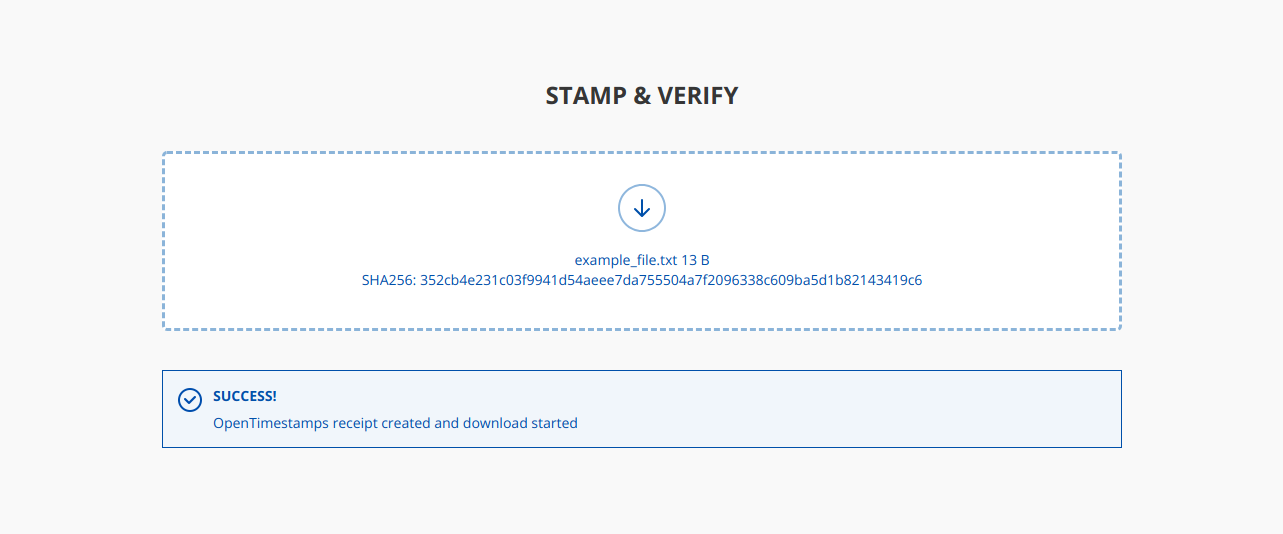
\includegraphics[width=1\linewidth]{Images/stamping.png}
	\caption{Stamping}
	\label{fig:ots-stamping}
\end{figure}

\newpage
\noindent
Alternatively, you can drop a \colorbox{light-gray}{.ots} file to \textit{verify}. Here the underlying code will detect if the file is yet in the \textit{incomplete} state and performs an \textit{upgrade}, automatically downloading the upgraded proof file. Otherwise, if the timestamp is already completed, it verifies such proof. Notice that the original document is required to start the verification process.

\bigskip
\begin{figure}[htbp]
    \centering
	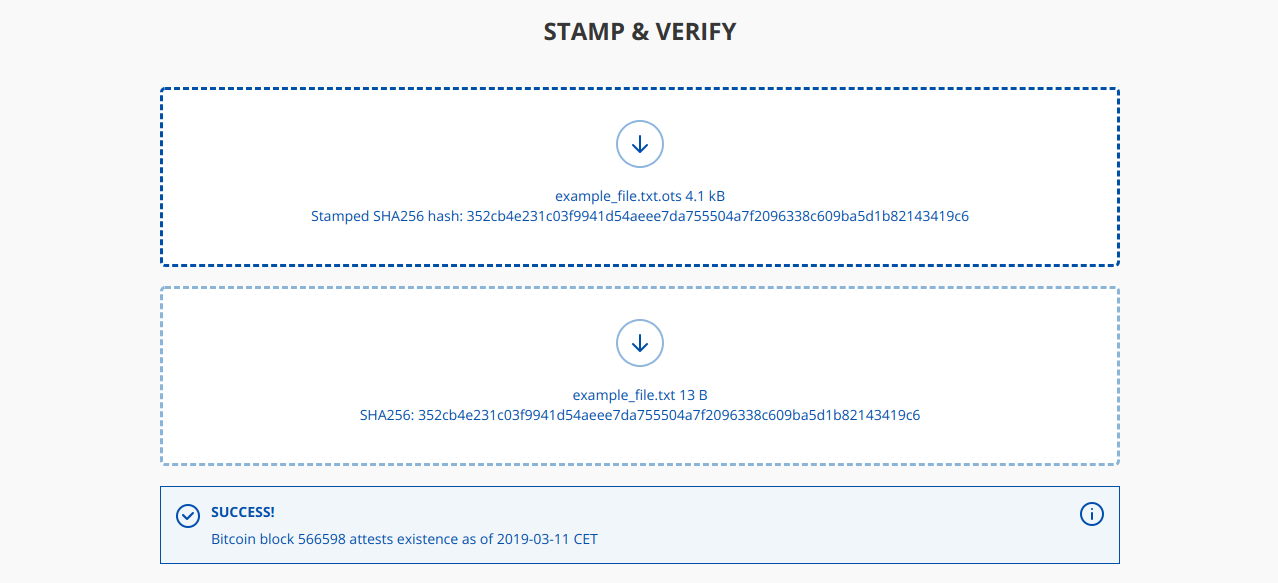
\includegraphics[width=1\linewidth]{Images/verify.png}
	\caption{Verifying}
	\label{fig:ots-verifying}
\end{figure}

\bigskip
\noindent
However, the web interface comes with a downside. Browsers applications like this one have some security restrictions, inhibiting a direct access to the local Bitcoin configuration file\footnote{We refer to Appendix \ref{app:A} for a detailed explanation about running a Bitcoin node, what RPC calls are and the main ones used in Bitcoin.}, thus preventing a user to make RPC calls to his own local Bitcoin node in order to verify a timestamp proof. Hence a user must trust the public block explorers that \textit{OpenTimestamps} uses to verify such proofs. Summing up, verification is not fully decentralized. Finally, clicking the \textit{info} button in the low right corner will open a new web page that parse the proof in a nice representation (like the \colorbox{light-gray}{info} command does for the client version, but with some added graphics).






\chapter{Blockchain Notarization: A Practical Use Case}
\label{chpr:project}
This Chapter is aimed to be a technical report of a project in which the author, in partnership with DGI (Digital Gold Institute) and ANIA (Associazione Nazionale fra le Imprese Assicuratrici), worked during the draft of this thesis.

\bigskip
\section{Executive Summary}
The purpose of this project work is to provide future clients a fully operating timestamping service, to enforce the notarization of digital documents which, as we already know, is traditionally achieved by certification authorities (CA), with a decentralized solution that is resilient even if the security of such CA is violated from the inside.

\bigskip
\noindent
The timestamping service is implemented, with some extensions and modification on the basis of need, according to the \textit{OpenTimestamps} protocol, because of its high scalability and low maintenance cost, all nice features that we already saw in the description of such protocol in Section \ref{sec:ots}. In addition, the proposed solution is independent of any provider, being \textit{OpenTimestamps} an open-source project. It could be made available to customers for free or in form of a subscription service, with specific service level agreements, in order to provide additional features like the custody of any user's timestamp proof. For example, any insurance company could make use of this solution to grant authenticity of its associates' insurance policies or, more generally, whenever a digital signature is involved. We remind that \textit{OpenTimestamps} also provides all the guarantees for an independent audit: a user can verify the validity of its timestamp proof without the need of the calendar server which actually maintains the service up, just by querying a local Bitcoin node or a public block explorer. Next we will move on the technical details regarding how this service is built, specifying when the \textit{OpenTimestamps} protocol is improved.

\bigskip
\section{Architecture of the Solution}
The architecture of the solution is composed by three servers (in cloud), accessible from outside via https thanks to network components.

\bigskip
\noindent
A user can easily connect to the public web server via browser at \url{https://timestamp.aniasafe.it} and drag a document to timestamp\footnote{We remind that what is really timestamped is the \textit{hash value} of such document, automatically computed on user's local device, without harming privacy. We refer to Chapter \ref{chpr:notarization} for all the details.}. It is directly from browser (thanks to the underlying JavaScript code) that the timestamp request is sent to the calendar servers to be processed. The corresponding timestamp proof is automatically downloaded on the user's local device and can be verified on the same web page, simply dragging the \colorbox{light-gray}{.ots} file. In that specific case, the browser will query public block explorers\footnote{As specified in Section \ref{sec:ots-web}, timestamping services deployed as browser applications cannot query a local Bitcoin node and have to trust public block explorers.} in order to perform the verification procedure. 

\bigskip
\noindent
Before getting into technical details regarding the code that underlies this solution, we present two explanatory figures. On one hand, Figure \ref{fig:ots-project-stamping} is aimed to give an abstract idea of the whole timestamping process, on the other hand Figure \ref{fig:ots-project-verifying} refers to the verification procedure.

\begin{figure}[ht]
    \centering
	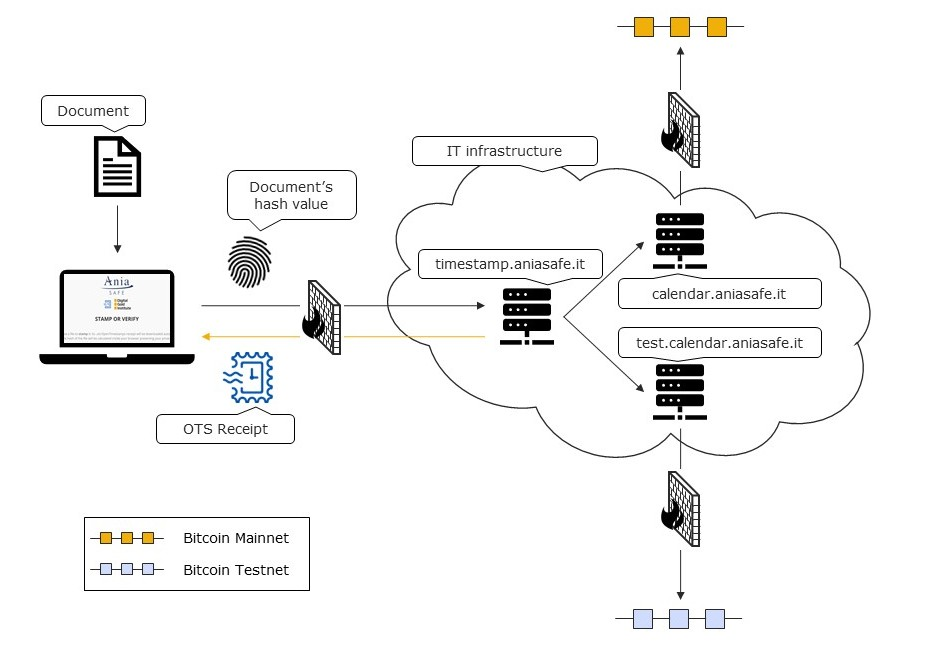
\includegraphics[width=1\linewidth]{Images/project-stamping.jpg}
	\caption{Architecture of the timestamping process}
	\label{fig:ots-project-stamping}
\end{figure}

\bigskip
\begin{figure}[ht]
    \centering
	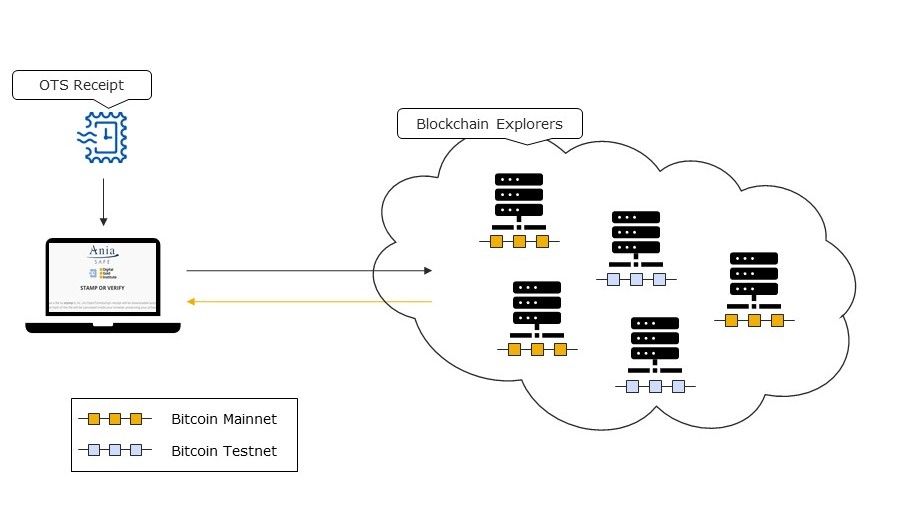
\includegraphics[width=1\linewidth]{Images/project-verifying.jpg}
	\caption{Architecture of the verification process}
	\label{fig:ots-project-verifying}
\end{figure}

\bigskip
\section{Technical Details}
The three servers introduced before are divided in a front-end server (\url{https://timestamp.aniasafe.it}) which hosts the public web page, and two back-end servers, the first one running a calendar server connected to a local\footnote{In the sense that the calendar server and the Bitcoin node run on the same machine.} Bitcoin node in mainnet mode (\url{https://calendar.aniasafe.it}), the latter connected to a local one in testnet mode (\url{https://test-calendar.aniasafe.it}).
\chapter{Conclusions}
\label{chpr:conclusions}


%----------------------------------------------------------------------------------------
%	THESIS CONTENT - APPENDICES
%----------------------------------------------------------------------------------------

\appendix
\chapter{Bitcoin from the command line}
\label{app:A}
This appendix is aimed at providing a technical walkthrough the Bitcoin network from the command line point of view, supposing a Unix-like operating system. Initially, we will configure a machine to launch a Bitcoin node; then we will introduce some of the most important RPC (taken from... metti la fonte) in order to perform basic operations. Lastly the OpenTimestamps protocol comes into play: we will practically see how to timestamp a document using the Python client and how to set up a calendar server.
\bigskip

\section{Running a Bitcoin Core node}
To get started with Bitcoin, you first need to join the network running a node. Following these simple steps will make the first experience a lot easier.
\begin{itemize}
\item Setup variables (for an easy installation):
\bigskip
\begin{lstlisting}
 $ export BITCOIN=bitcoin-core-0.17.0
\end{lstlisting}
\item Download relevant files (Remark: every time you find username replace it with your personal one):
\bigskip
\begin{lstlisting}
 $ wget https://bitcoin.org/bin/$BITCOIN/$BITCOINPLAIN-x86_64-linux-gnu.tar.gz -O ~username/$BITCOINPLAIN-x86_64-linux-gnu.tar.gz
 $ wget https://bitcoin.org/bin/$BITCOIN/SHA256SUMS.asc -O ~username/SHA256SUMS.asc
 $ wget https://bitcoin.org/laanwj-releases.asc -O ~username/laanwj-releases.asc
\end{lstlisting}
\item Verify Bitcoin signature (in order to verify that your Bitcoin setup is authentic):
\bigskip
\begin{lstlisting}
 $ /usr/bin/gpg --import ~username/laanwj-releases.asc
 $ /usr/bin/gpg --verify ~username/SHA256SUMS.asc
\end{lstlisting}
Amongst the info you get back from the last command should be a line telling \enquote{Good signature}, do not care the rest.
\item Verify Bitcoin SHA (Secure Hash Algorithm) of the .tar file against the expected one:
\bigskip
\begin{lstlisting}
 $ /usr/bin/sha256sum ~username/$BITCOINPLAIN-x86_64-linux-gnu.tar.gz | awk '{print $1}'
 $ cat ~username/SHA256SUMS.asc | grep $BITCOINPLAIN-x86_64-linux-gnu.tar.gz | awk '{print $1}'
\end{lstlisting}
From this verification you must obtain the same number.
\item Install Bitcoin:
\bigskip
\begin{lstlisting}
 $ /bin/tar xzf ~username/$BITCOINPLAIN-x86_64-linux-gnu.tar.gz -C ~username
 $ sudo /usr/bin/install -m 0755 -o root -g root -t /usr/local/bin ~username/$BITCOINPLAIN/bin/*
 $ /bin/rm -rf ~username/$BITCOINPLAIN/
\end{lstlisting}
\item Create the configuration file:

\bigskip
\noindent
First, create the directory you want to put your data into: \bigskip
\begin{lstlisting}
 $ /bin/mkdir ~username/.bitcoin
\end{lstlisting}
Then create the configuration file (as you need it):
\bigskip
\begin{lstlisting}
 $ cat >> ~username/.bitcoin/bitcoin.conf << EOF
 # Accept command line and JSON-RPC commands
 server=1
 # Username for JSON-RPC connections
 rpcuser=invent_a_username_here
 # Password for JSON-RPC connections
 rpcpassword=invent_a_long_pwd_here
 # Enable Testnet chain mode
 testnet=1
 EOF
\end{lstlisting}
The \textit{bitcoin.conf} file is the default file which Bitcoin daemon reads when launched, and it contains instructions to configure the node (e.g. mainnet, testnet or regtest mode). In this example we define a \textit{rpcuser} and \textit{rpcpassword} to enable RPC, and we tell the node to synchronize with the Bitcoin Testnet chain. (metti una nota qui per il sito dei conf file).

\bigskip
\noindent
Finally, limit the permissions to your configuration file (not really needed, but more secure): \bigskip
\begin{lstlisting}
 $ /bin/chmod 600 ~username/.bitcoin/bitcoin.conf
\end{lstlisting}
\item Start the daemon\footnote{In multitasking computer operating systems, a \textit{daemon} is a computer program that runs as a background process, rather than being under direct control of an interactive user. Traditionally, the process names of a daemon end with the letter \textit{d}; \colorbox{Grey!10}{bitcoind} is the one which implements the Bitcoin protocol for remote procedure call (RPC) use.}:
\bigskip
\begin{lstlisting}
 $ bitcoind -daemon
\end{lstlisting}
\end{itemize}
We are now ready to be part of the Bitcoin network ! \\ 
In the next section we will learn how to manage the Bitcoin command line interface.

\bigskip

\section{Bitcoin-cli: command line interface}
In this section we will answer the following question: \enquote{\textit{What is RPC and which calls are the most used in Bitcoin?}}.

\bigskip
\noindent
Without further going into details regarding computer science\footnote{For more details, see \url{https://en.wikipedia.org/wiki/Remote\_procedure\_call}.}, a RPC (Remote Procedure Call) is a powerful technique for constructing distributed, client-server based applications. It is based on the extension of the conventional procedure calling, so that the called procedure need not exist in the same address space as the calling procedure. The two processes may be on the same system, or they may be on different systems with a network connecting them. Our interest is for the \colorbox{Grey!10}{bitcoin-cli}, a handy interface that lets the user send commands to the \colorbox{Grey!10}{bitcoind}. More specifically, it lets you send RPC commands to the \colorbox{Grey!10}{bitcoind}. Generally, the \colorbox{Grey!10}{bitcoin-cli} interface is much more clean and user friendly than trying to send RPC commands by hand, using \colorbox{Grey!10}{curl} or some other method.

\bigskip
\noindent
The first thing to do for a beginner user is to look for the full list of calls invoking the \colorbox{Grey!10}{help} command:
\bigskip
\begin{lstlisting}
 $ bitcoin-cli help
 
 == Blockchain ==
 getbestblockhash
 getblock "blockhash" ( verbosity ) 
 getblockchaininfo
 getblockcount
 getblockhash height
 getblockheader "hash" ( verbose )
 getblockstats hash_or_height ( stats )
 getchaintips
 getchaintxstats ( nblocks blockhash )
 getdifficulty
 getmempoolancestors txid (verbose)
 getmempooldescendants txid (verbose)
 getmempoolentry txid
 getmempoolinfo
 getrawmempool ( verbose )
 gettxout "txid" n ( include_mempool )
 gettxoutproof ["txid",...] ( blockhash )
 gettxoutsetinfo
 preciousblock "blockhash"
 pruneblockchain
 savemempool
 scantxoutset <action> ( <scanobjects> )
 verifychain ( checklevel nblocks )
 verifytxoutproof "proof"

 == Control ==
 getmemoryinfo ("mode")
 help ( "command" )
 logging ( <include> <exclude> )
 stop
 uptime

 == Generating ==
 generate nblocks ( maxtries )
 generatetoaddress nblocks address (maxtries)

 == Mining ==
 getblocktemplate ( TemplateRequest )
 getmininginfo
 getnetworkhashps ( nblocks height )
 prioritisetransaction <txid> <dummy value> <fee delta>
 submitblock "hexdata"  ( "dummy" )

 == Network ==
 addnode "node" "add|remove|onetry"
 clearbanned
 disconnectnode "[address]" [nodeid]
 getaddednodeinfo ( "node" )
 getconnectioncount
 getnettotals
 getnetworkinfo
 getpeerinfo
 listbanned
 ping
 setban "subnet" "add|remove" (bantime) (absolute)
 setnetworkactive true|false

 == Rawtransactions ==
 combinepsbt ["psbt",...]
 combinerawtransaction ["hexstring",...]
 converttopsbt "hexstring" ( permitsigdata iswitness )
 createpsbt [{"txid":"id","vout":n},...] [{"address":amount},{"data":"hex"},...] ( locktime ) ( replaceable )
 createrawtransaction [{"txid":"id","vout":n},...] [{"address":amount},{"data":"hex"},...] ( locktime ) ( replaceable )
 decodepsbt "psbt"
 decoderawtransaction "hexstring" ( iswitness )
 decodescript "hexstring"
 finalizepsbt "psbt" ( extract )
 fundrawtransaction "hexstring" ( options iswitness )
 getrawtransaction "txid" ( verbose "blockhash" )
 sendrawtransaction "hexstring" ( allowhighfees )
 signrawtransaction "hexstring" ( [{"txid":"id","vout":n,"scriptPubKey":"hex","redeemScript":"hex"},...] ["privatekey1",...] sighashtype )
 signrawtransactionwithkey "hexstring" ["privatekey1",...] ( [{"txid":"id","vout":n,"scriptPubKey":"hex","redeemScript":"hex"},...] sighashtype )
 testmempoolaccept ["rawtxs"] ( allowhighfees )

 == Util ==
 createmultisig nrequired ["key",...] ( "address_type" )
 estimatesmartfee conf_target ("estimate_mode")
 signmessagewithprivkey "privkey" "message"
 validateaddress "address"
 verifymessage "address" "signature" "message"

 == Wallet ==
 abandontransaction "txid"
 abortrescan
 addmultisigaddress nrequired ["key",...] ( "label" "address_type" )
 backupwallet "destination"
 bumpfee "txid" ( options ) 
 createwallet "wallet_name" ( disable_private_keys )
 dumpprivkey "address"
 dumpwallet "filename"
 encryptwallet "passphrase"
 getaccount (Deprecated, will be removed in V0.18. To use this command, start bitcoind with -deprecatedrpc=accounts)
 getaccountaddress (Deprecated, will be removed in V0.18. To use this command, start bitcoind with -deprecatedrpc=accounts)
 getaddressbyaccount (Deprecated, will be removed in V0.18. To use this command, start bitcoind with -deprecatedrpc=accounts)
 getaddressesbylabel "label"
 getaddressinfo "address"
 getbalance ( "(dummy)" minconf include_watchonly )
 getnewaddress ( "label" "address_type" )
 getrawchangeaddress ( "address_type" )
 getreceivedbyaccount (Deprecated, will be removed in V0.18. To use this command, start bitcoind with -deprecatedrpc=accounts)
 getreceivedbyaddress "address" ( minconf )
 gettransaction "txid" ( include_watchonly )
 getunconfirmedbalance
 getwalletinfo
 importaddress "address" ( "label" rescan p2sh )
 importmulti "requests" ( "options" )
 importprivkey "privkey" ( "label" ) ( rescan )
 importprunedfunds
 importpubkey "pubkey" ( "label" rescan )
 importwallet "filename"
 keypoolrefill ( newsize )
 listaccounts (Deprecated, will be removed in V0.18. To use this command, start bitcoind with -deprecatedrpc=accounts)
 listaddressgroupings
 listlabels ( "purpose" )
 listlockunspent
 listreceivedbyaccount (Deprecated, will be removed in V0.18. To use this command, start bitcoind with -deprecatedrpc=accounts)
 listreceivedbyaddress ( minconf include_empty include_watchonly address_filter )
 listsinceblock ( "blockhash" target_confirmations include_watchonly include_removed )
 listtransactions (dummy count skip include_watchonly)
 listunspent ( minconf maxconf  ["addresses",...] [include_unsafe] [query_options])
 listwallets
 loadwallet "filename"
 lockunspent unlock ([{"txid":"txid","vout":n},...])
 move (Deprecated, will be removed in V0.18. To use this command, start bitcoind with -deprecatedrpc=accounts)
 removeprunedfunds "txid"
 rescanblockchain ("start_height") ("stop_height")
 sendfrom (Deprecated, will be removed in V0.18. To use this command, start bitcoind with -deprecatedrpc=accounts)
 sendmany "" {"address":amount,...} ( minconf "comment" ["address",...] replaceable conf_target "estimate_mode")
 sendtoaddress "address" amount ( "comment" "comment_to" subtractfeefromamount replaceable conf_target "estimate_mode")
 setaccount (Deprecated, will be removed in V0.18. To use this command, start bitcoind with -deprecatedrpc=accounts)
 sethdseed ( "newkeypool" "seed" )
 settxfee amount
 signmessage "address" "message"
 signrawtransactionwithwallet "hexstring" ( [{"txid":"id","vout":n,"scriptPubKey":"hex","redeemScript":"hex"},...] sighashtype )
 unloadwallet ( "wallet_name" )
 walletcreatefundedpsbt [{"txid":"id","vout":n},...] [{"address":amount},{"data":"hex"},...] ( locktime ) ( replaceable ) ( options bip32derivs )
 walletlock
 walletpassphrase "passphrase" timeout
 walletpassphrasechange "oldpassphrase" "newpassphrase"
 walletprocesspsbt "psbt" ( sign "sighashtype" bip32derivs )

 == Zmq ==
 getzmqnotifications
\end{lstlisting}

\bigskip
\noindent
You can also type \colorbox{Grey!10}{bitcoin-cli help [command]} to be even more extensive about that command. For example:
\bigskip
\begin{lstlisting}
 $ bitcoin-cli help getmininginfo
 
 getmininginfo

 Returns a json object containing mining-related information.
 Result:
 {
   "blocks": nnn,             (numeric) The current block
   "currentblockweight": nnn, (numeric) The last block weight
   "currentblocktx": nnn,     (numeric) The last block transaction
   "difficulty": xxx.xxxxx    (numeric) The current difficulty
   "networkhashps": nnn,      (numeric) The network hashes per second
   "pooledtx": n              (numeric) The size of the mempool
   "chain": "xxxx",           (string) current network name as defined in BIP70 (main, test, regtest)
   "warnings": "..."          (string) any network and blockchain warnings
 }

 Examples:
 > bitcoin-cli getmininginfo 
 > curl --user myusername --data-binary '{"jsonrpc": "1.0", "id":"curltest", "method": "getmininginfo", "params": [] }' -H 'content-type: text/plain;' http://127.0.0.1:8332/
\end{lstlisting}
\bigskip
\noindent
Here is a list of the most general commands to get additional information about bitcoin data:
\bigskip
\begin{lstlisting}
 $ bitcoin-cli getblockchaininfo
 $ bitcoin-cli getmininginfo
 $ bitcoin-cli getnetworkinfo
 $ bitcoin-cli getnettotals
 $ bitcoin-cli getwalletinfo
\end{lstlisting}
\bigskip
\noindent
For example \colorbox{Grey!10}{bitcoin-cli getwalletinfo} gives the user precise information about the bitcoin wallet, like the confirmed and unconfirmed balance (nota a pie' pagina per spiegare cosa sia unconfirmed balance), and the total number of transactions in the wallet.
\bigskip
\begin{lstlisting}
 $ bitcoin-cli getwalletinfo
 {
  "walletname": "",
  "walletversion": 169900,
  "balance": 0.07825304,
  "unconfirmed_balance": 0.00000000,
  "immature_balance": 0.00000000,
  "txcount": 1,
  "keypoololdest": 1544714806,
  "keypoolsize": 999,
  "keypoolsize_hd_internal": 1000,
  "paytxfee": 0.00000000,
  "hdseedid": "972e6ac8d0104fec0d0e6c052d3876ada965c745",
  "hdmasterkeyid": "972e6ac8d0104fec0d0e6c052d3876ada965c745",
  "private_keys_enabled": true
}
\end{lstlisting}





\backmatter
%----------------------------------------------------------------------------------------
%	BIBLIOGRAPHY
%----------------------------------------------------------------------------------------

\backmatter
\nocite{*}
\bibliographystyle{acm}
\bibliography{Bibliography/bibliography}



\end{document}  